% arara: latex: { interaction: nonstopmode, options: ['-halt-on-error'] }
% arara: dvisvgm: { options: ['--no-fonts', '--exact-bbox', '--zoom=-1'] }
% The order shown is one possible result of the initial random shuffle.
\documentclass[tikz,border=8pt,11pt]{standalone}
\usepackage{amsmath}
\definecolor{circleblue}{HTML}{0072B2}
\definecolor{pointred}{HTML}{D55E00}
\definecolor{ink}{HTML}{25313C}
\definecolor{muted}{HTML}{7C8792}
\tikzset{
  current/.style={draw=circleblue,line width=1.1pt,fill=circleblue!6},
  previous/.style={draw=muted,dashed,line width=0.9pt},
  point label/.style={font=\small,inner sep=3pt,text=ink},
}

% Arguments: number of inserted points; most recently inserted point.
% Coordinates and label anchors are identical in all panels.
\newcommand{\points}[2]{%
  \foreach \id/\px/\py/\anchor in {
    1/-2/0/north east,2/2/0/north west,3/0/1/west,4/0/3/south}{%
    \ifnum\id>#1\relax
      \draw[muted,fill=white,line width=0.7pt] (\px,\py) circle[radius=2.3pt];
      \node[point label,text=muted,anchor=\anchor] at (\px,\py) {$P_{\id}$};
    \else
      \ifnum\id=#2\relax
        \fill[pointred] (\px,\py) circle[radius=3pt];
        \node[point label,text=pointred,anchor=\anchor] at (\px,\py) {$P_{\id}$};
      \else
        \fill[ink] (\px,\py) circle[radius=2.3pt];
        \node[point label,anchor=\anchor] at (\px,\py) {$P_{\id}$};
      \fi
    \fi
  }%
}

\begin{document}
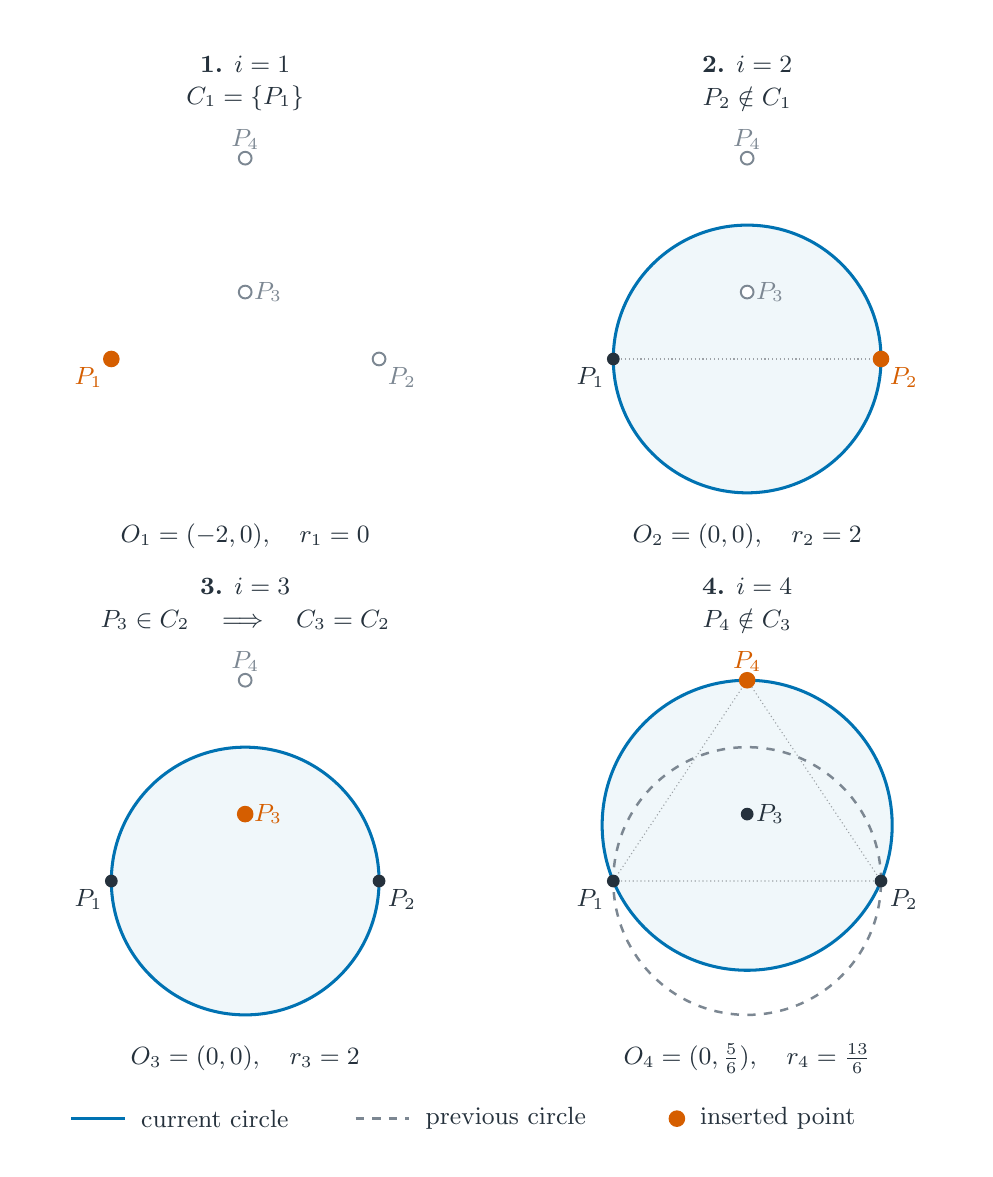
\begin{tikzpicture}[x=0.85cm,y=0.85cm,font=\small,text=ink]
  % White background also keeps the diagram legible in dark themes.
  \fill[white] (-3.25,-11.8) rectangle (10.75,4.95);

  \begin{scope}
    \node at (0,4.4) {\textbf{1.} $i=1$};
    \node at (0,3.9) {$C_1=\{P_1\}$};
    \points{1}{1}
    \node at (0,-2.65) {$O_1=(-2,0),\quad r_1=0$};
  \end{scope}

  \begin{scope}[xshift=6.375cm]
    \node at (0,4.4) {\textbf{2.} $i=2$};
    \node at (0,3.9) {$P_2\notin C_1$};
    \draw[current] (0,0) circle[radius=2];
    \draw[ink!45,densely dotted] (-2,0) -- (2,0);
    \points{2}{2}
    \node at (0,-2.65) {$O_2=(0,0),\quad r_2=2$};
  \end{scope}

  \begin{scope}[yshift=-6.63cm]
    \node at (0,4.4) {\textbf{3.} $i=3$};
    \node at (0,3.9) {$P_3\in C_2\quad\Longrightarrow\quad C_3=C_2$};
    \draw[current] (0,0) circle[radius=2];
    \points{3}{3}
    \node at (0,-2.65) {$O_3=(0,0),\quad r_3=2$};
  \end{scope}

  \begin{scope}[xshift=6.375cm,yshift=-6.63cm]
    \node at (0,4.4) {\textbf{4.} $i=4$};
    \node at (0,3.9) {$P_4\notin C_3$};
    \draw[current] (0,{5/6}) circle[radius={13/6}];
    \draw[previous] (0,0) circle[radius=2];
    \draw[ink!45,densely dotted] (-2,0) -- (2,0) -- (0,3) -- cycle;
    \points{4}{4}
    \node at (0,-2.65) {$O_4=(0,\tfrac56),\quad r_4=\tfrac{13}{6}$};
  \end{scope}

  \draw[circleblue,line width=1.1pt] (-2.6,-11.35) -- (-1.8,-11.35);
  \node[anchor=west] at (-1.7,-11.35) {current circle};
  \draw[previous] (1.65,-11.35) -- (2.45,-11.35);
  \node[anchor=west] at (2.55,-11.35) {previous circle};
  \fill[pointred] (6.45,-11.35) circle[radius=3pt];
  \node[anchor=west] at (6.65,-11.35) {inserted point};
\end{tikzpicture}
\end{document}
